\documentclass[12pt]{article}
\textwidth 15.5cm \oddsidemargin 0cm \topmargin -1cm \textheight
24cm \footskip 1.5cm \usepackage{epsfig}
\usepackage{amsmath,graphicx,psfrag,pstcol}
\usepackage{xcolor}
\usepackage{subfigure}
\usepackage{listings}
\def\n{\noindent}
\def\u{\underline}
\def\hs{\hspace}
\newcommand{\thrfor}{.^{\displaystyle .} .}
\newcommand{\bvec}[1]{{\bf #1}}
\graphicspath{{/Users/ranshanzi/Desktop/figures/}}

\definecolor{darkblue}{RGB}{0, 0, 139}

\begin{document}

\noindent
\rule{15.7cm}{0.5mm}


\begin{center}
{\bf ENGINEERING TRIPOS PART II A}
\end{center}
\vspace{0.5cm} {\bf EIETL \hfill MODULE EXPERIMENT 3F3}
\vspace{0.5cm}
\begin{center}
{\bf RANDOM VARIABLES and RANDOM NUMBER GENERATION\\
Short  Report Template\\\hfill \\Name: Shanzi (Monica) Ran\\\hfill\\
College: Magdalene College\\\hfill
\\
}
\end{center}
\rule{15.7cm}{0.5mm}



\vspace*{1cm}
\begin{center}
\fbox{\parbox{0.8\linewidth}{\bf This  is a template suitable for the short report write-up. Simply edit the Latex or Word document to include your calculations/ results/ code.}}
\end{center}
\vspace*{1cm}

\begin{enumerate}
\item {\bf Uniform and normal random variables.}

Histogram of Gaussian random numbers overlaid on exact Gaussian curve (scaled):
\begin{figure}[h]
    \centering
    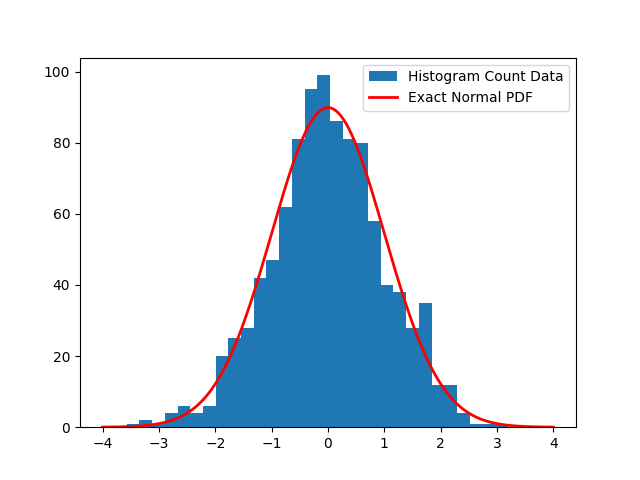
\includegraphics[width=0.6\textwidth]{q1_1}
    \caption{Histogram of Gaussian random numbers overlaid on exact Gaussian curve}
    \label{fig:q1_1}
\end{figure}
\vspace{3in}

Histogram of Uniform random numbers overlaid on exact Uniform curve (scaled):
\begin{figure}[h]
    \centering
    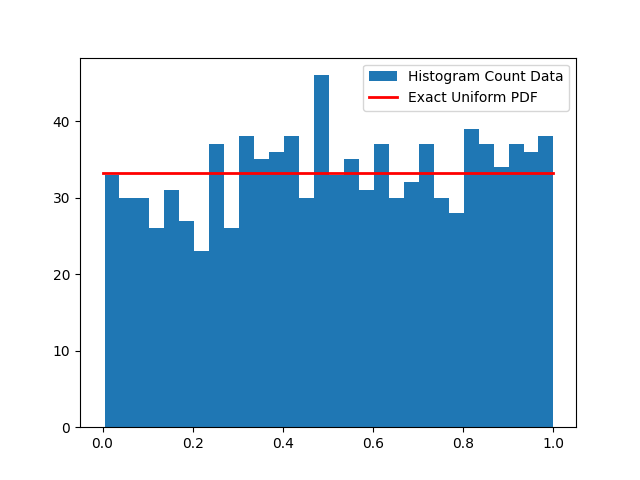
\includegraphics[width=0.6\textwidth]{q1_2}
    \caption{Histogram of Uniform random numbers overlaid on exact Uniform curve}
    \label{fig:q1_2}
\end{figure}
\vspace{1in}

Kernel density estimate for Gaussian random numbers overlaid on exact Gaussian curve:
\begin{figure}[h]
    \centering
    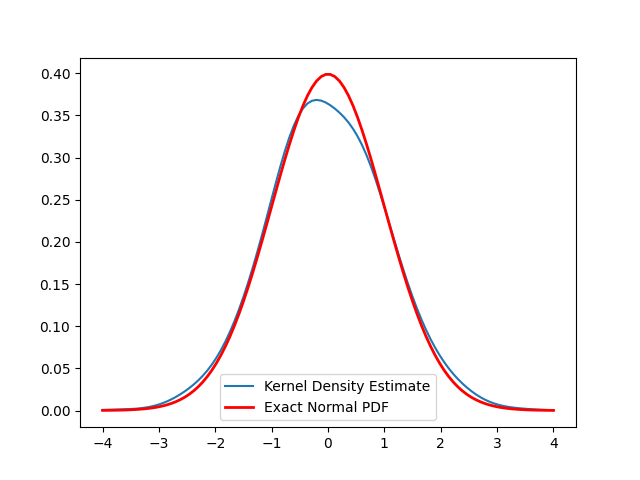
\includegraphics[width=0.6\textwidth]{q1_3}
    \caption{Kernel density estimate for Gaussian random numbers overlaid on exact Gaussian curve}
    \label{fig:q1_3}
\end{figure}
\vspace{3in}



Kernel density estimate for Uniform random numbers overlaid on exact Gaussian curve:
\begin{figure}[h]
    \centering
    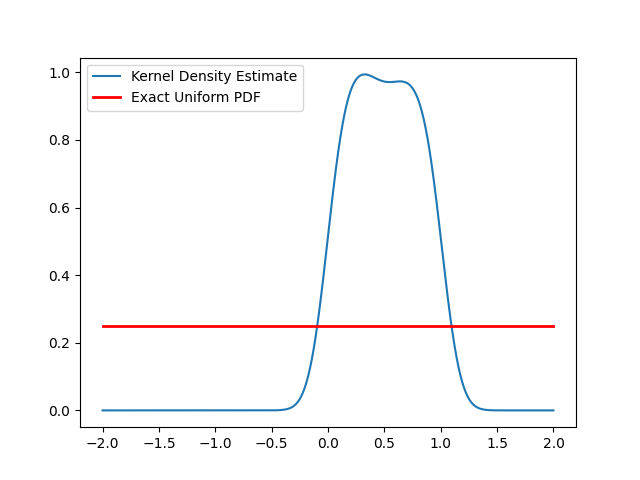
\includegraphics[width=0.6\textwidth]{q1_4}
    \caption{Kernel density estimate for Uniform random numbers overlaid on exact Gaussian curve}
    \label{fig:q1_4}
\end{figure}
\vspace{1.5in}

Comment on the advantages and disadvantages of the kernel density method compared with the histogram method for estimation of a probability density from random samples:

\textcolor{darkblue}{Kernel Density Method (KDE) gives an estimation with a more continuous presentation due to its smoothing function, while histogram presentations are better for discrete data.\\
\\
On the other hand, KDE requires a careful choice of the operation bandwidth as overfitting (bandwith too small, estimation not representative of original data) or underfitting (bandwidth too small, estimation very spiky and difficult for statistical analysis) are highly likely. Therefore, histograms are generally more intuitive and robust to bandwidth selection.}
\vspace{3in}



Theoretical  mean and standard deviation calculation for uniform density as a function of $N$:
\textcolor{darkblue}{
    \begin{flushleft} % Left-align the entire block
        \begin{align*}
            & X \sim \mathcal{U}(0,1) \\
            & \text{Assume histogram has } j \text{ bins, for } N \text{ random variables.} \\
            & \text{Since } \sum_{i=0}^{j} p_i = 1, \quad p_i = \frac{1}{j}. \\
            & \text{Mean per bin: } N p_j = \frac{N}{j}. \\
            & \text{Variance per bin: } N p_j (1 - p_j) = \frac{N}{j} \left( 1 - \frac{1}{j} \right). \\
            & \text{Uniform distribution implies mean and variance are the same for each bin.} \\
            & \text{Overall (summed up): } \text{Mean} = \frac{N}{j} \propto N, \quad \text{Standard deviation} = \sqrt{\frac{N}{j} \left( 1 - \frac{1}{j} \right)} \propto \sqrt{N}.
        \end{align*}
    \end{flushleft}
}
\vspace{2in}

Explain behaviour as $N$ becomes large:
\textcolor{darkblue}{
    \begin{flushleft} % Left-align the entire block
        \begin{align*}
            & \text{From above, }\\ 
            & \text{overall mean}=\frac{N}{j}\propto N\\
            & \text{overall standard deviation}=\sqrt{\frac{N}{j}(1-\frac{1}{j})}\propto \sqrt{N}\\
            & \text{so as N grow large, mean of histogram count grows at}N\text{, standard deviation grows at}N\sqrt{N}\text{.}
        \end{align*}
    \end{flushleft}
}
\vspace{3in}



Plot of histograms for $N=100$,  $N=1000$ and $N=10000$ with theoretical mean  and $\pm 3$ standard deviation lines:
\begin{figure}[htbp]
    \centering
    \subfigure[N=100]{
        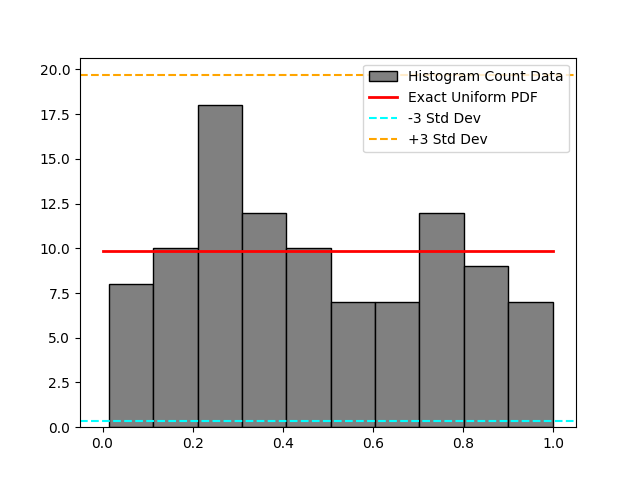
\includegraphics[width=0.3\textwidth]{q1_5_100_bin_10}
        \label{fig:q1_5_1}
    }
    \subfigure[N=1000]{
        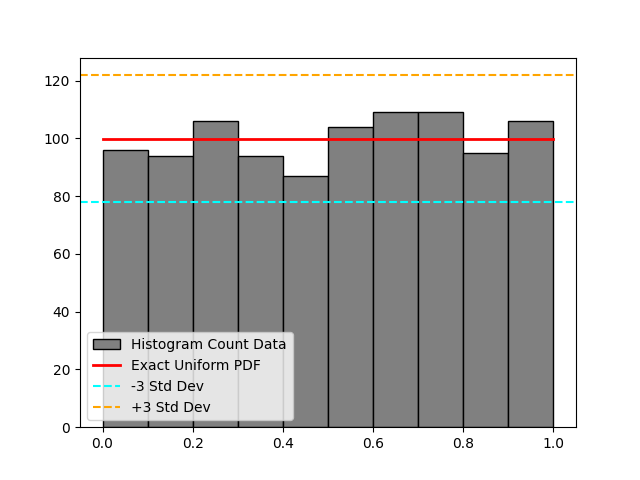
\includegraphics[width=0.3\textwidth]{q1_5_1000_bin_10}
        \label{fig:q1_5_2}
    }
    \subfigure[N=10000]{
        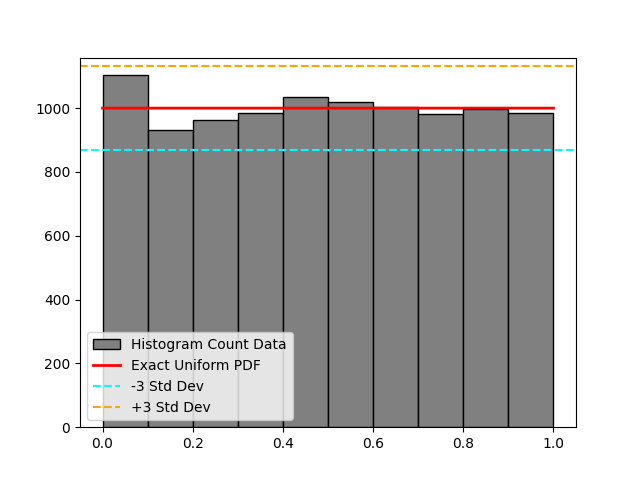
\includegraphics[width=0.3\textwidth]{q1_5_10000_bin_10}
        \label{fig:q1_5_3}
    }
    \caption{Histograms for different values of N with theoretical mean and standard deviation lines}
    \label{fig:q1_5}
\end{figure}
\vspace{3in}

 Are your histogram results consistent with the multinomial distribution theory? 

 \textcolor{darkblue}{
    As shown in Figure~\ref{fig:q1_5}, the mean of histogram count data approaches the theoretical value (marked by the red horizontal line) as N grows larger.
    The standard deviation of the sampled data points is also shrinking, indicating that the distribution of bin counts is more uniform than before.
    Therefore, the histogram results in Figure~\ref{fig:q1_5} is consistent with the multinomial distribution theory from which the mean and standard deviation formula for each bin j is developed from.
}
\vspace{3in}


\item {\bf Functions of random variables}
For normally distributed ${\cal N}(x|0,1)$ random variables, take $y=f(x)=ax+b$. Calculate $p(y)$ using the Jacobian formula:
\textcolor{darkblue}{
    \begin{flalign*}
        & X \sim \mathcal{N}(0,1) & \\
        & y = f(x) = ax + b \text{, so } x = f^{-1}(y) = \frac{y - b}{a} & \\
        & \frac{dy}{dx} = a & \\
        & \begin{aligned}
            p(y) &= \frac{p(x)}{\left|\frac{dy}{dx}\right|}\Big|_{x=f^{-1}(y)} \\
                 &= \frac{1}{a} p\left(\frac{y - b}{a}\right)\\
                 &= \frac{1}{\sqrt{2\pi }a}exp(-\frac{1}{2}(\frac{y-b}{a})^2)
        \end{aligned} &
    \end{flalign*}
}
\vspace{2in}

Explain how this is linked to the general normal density with non-zero mean and non-unity variance:
\textcolor{darkblue}{
    \begin{flalign*}
        & \text{Compare the pdf of this transformed \( y \) with that of a standard normal, it is observed that:} &
    \end{flalign*}
}
\textcolor{darkblue}{
    \begin{center}
        $\mu = b, \quad \sigma= a$
    \end{center}
}
\textcolor{darkblue}{
    \begin{flalign*}
        & \text{This indicate that y corresponds to a normal density distribution with mean}=b, \text{variance}=a^2.
    \end{flalign*}
}

\vspace{3in}



 Verify this formula by transforming a large collection of random samples $x^{(i)}$ to give $y^{(i)}=f(x^{(i)})$, histogramming the resulting $y$ samples, and overlaying a plot of your formula calculated using the Jacobian:
\begin{figure}[h]
    \centering
    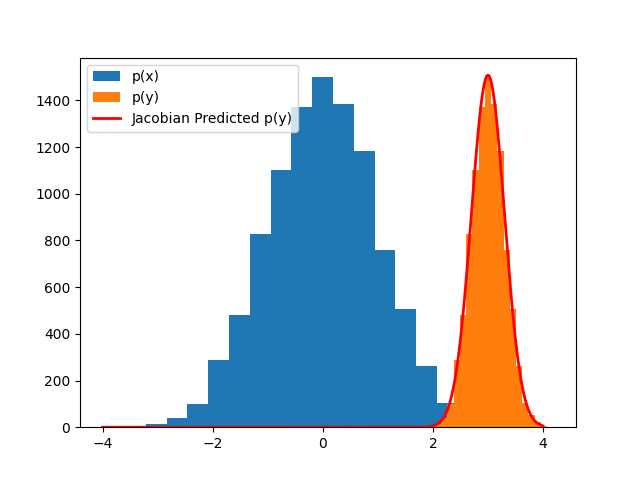
\includegraphics[width=0.6\textwidth]{q2_1}
    \caption{Sampled transformation for y=ax+b}
    \label{fig:q2_1}
\end{figure}
\vspace{1in}

Now take $p(x)={\cal N}(x|0,1)$ and $f(x)=x^2$. Calculate $p(y)$ using the Jacobian formula:
\textcolor{darkblue}{
    \begin{flalign*}
        & X \sim \mathcal{N}(0,1) & \\
        & y = f(x) = x ^ 2 \text{, so } x = f^{-1}(y) = \pm \sqrt{y} \text{ , where } x_1 = \sqrt{y},\: x_2 = -\sqrt{y}& \\
        & \frac{dy}{dx} = 2x & \\
        & \begin{aligned}
            p(y) &= \sum_{k=1}^{2}\frac{p(x)}{|\frac{dy}{dx}|}\big|_{x=x_k(y)}& \\
                 &= \frac{1}{\sqrt{2\pi}}exp(-\frac{y}{2})(\frac{1}{2\sqrt{y}}+|\frac{1}{2\sqrt{y}}|)& \\
                 &= \frac{1}{\sqrt{2\pi y}}exp(-\frac{y}{2})
        \end{aligned} &
    \end{flalign*}
}
\vspace{3in}




 Verify your result by histogramming of transformed random samples:
 \begin{figure}[h]
    \centering
    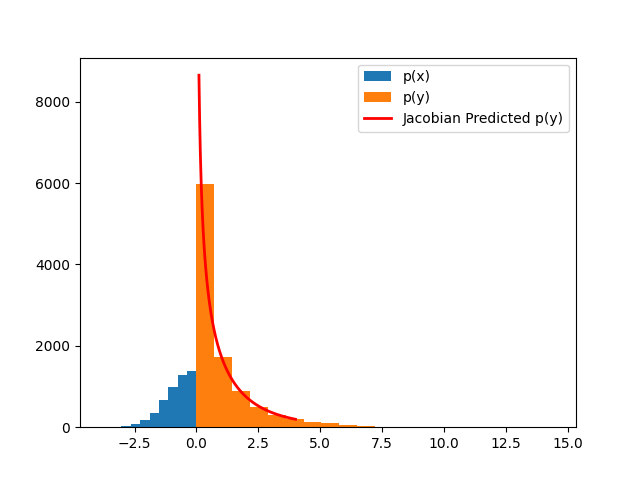
\includegraphics[width=0.6\textwidth]{q2_2}
    \caption{Sampled transformation for $y=x^2$}
    \label{fig:q2_2}
\end{figure}
\vspace{6in}


\item{\bf Inverse CDF method} 



Calculate the CDF and the inverse CDF for the exponential distribution: 
\textcolor{darkblue}{
    \begin{flalign*}
        & p(y) = \frac{df^{-1}(y)}{dy} = \exp(-y) & \\
        & \begin{aligned}
            \text{CDF: By definition of CDF, } F(y) &= \int_{0}^{y} p(y) \, dy &\\ 
            &= \int_{0}^{y} \exp(-y) \, dy &\\
            &= 1 - \exp(-y) &\\
        \end{aligned} &\\
        & \begin{aligned}
            \text{Inverse CDF: } &y = f(x) \; x = f^{-1}(y) &\\
                                 &\text{From CDF, } x = 1 - e^{-y} &\\
                                 & F^{-1}(x) = f(x) = y = -\ln(1-x) &
        \end{aligned} &\\
    \end{flalign*}
}
\vspace{3in}



Matlab/Python code for inverse CDF method for generating samples from the exponential distribution:
\begin{lstlisting}[language=Python, basicstyle=\ttfamily\small, keywordstyle=\color{blue}]
    import numpy as np
    
    def inverse_cdf(n, exp_lambda):
        x = np.random.rand(n)
        samples = - np.log(1 - x) / exp_lambda
        return samples
\end{lstlisting}
\vspace{3in}



Plot histograms/ kernel density estimates and overlay them on the desired exponential density:
\begin{figure}[h]
    \centering
    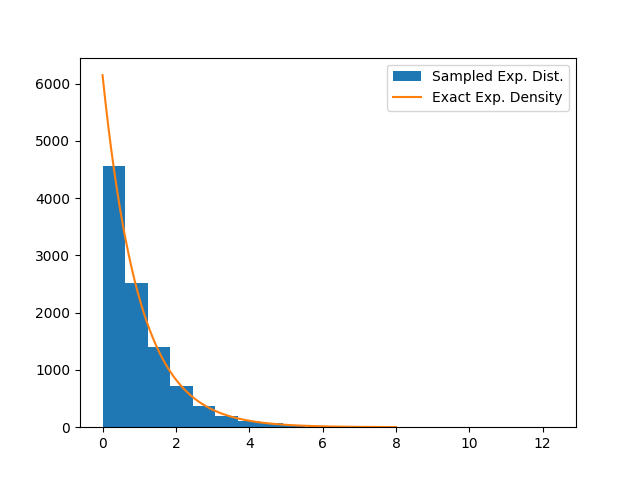
\includegraphics[width=0.6\textwidth]{q3_1_hist}
    \caption{Generating samples from exponential distribution (histogram)}
    \label{fig:q3_1_hist}
\end{figure}
\begin{figure}[h]
    \centering
    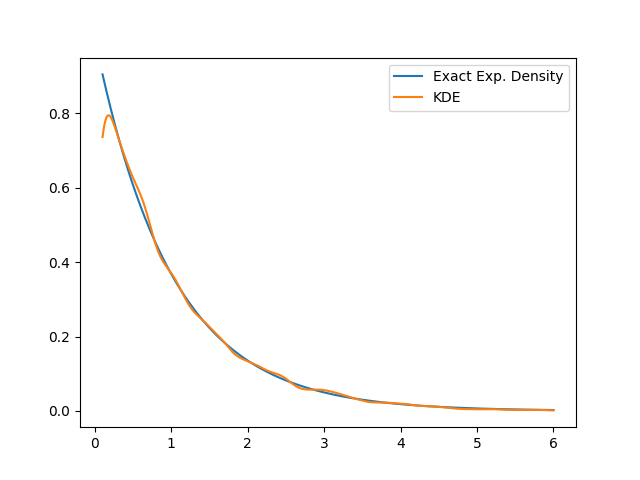
\includegraphics[width=0.6\textwidth]{q3_1_kde}
    \caption{Generating samples from exponential distribution (KDE)}
    \label{fig:q3_1_kde}
\end{figure}
\vspace{3in}

\item {\bf Simulation from a `non-standard'  density.}

Matlab/Python code to generate $N$ random numbers drawn from the distribution of $X$:
\begin{lstlisting}[language=Python, basicstyle=\ttfamily\small, keywordstyle=\color{blue}, breaklines=true]
    import numpy as np
    
    def gen_x(n, alpha, beta):
        b = np.arctan(beta * np.tan(np.pi * alpha / 2)) / alpha
        s = (1 + (beta ** 2) * (np.tan(np.pi * alpha / 2) ** 2)) ** (1 / (2 * alpha))

        u = np.random.uniform(low=(-np.pi/2), high=(np.pi/2), size=n)
        v = np.random.exponential(scale=1, size=n)

        x = s * np.sin(alpha * (u + b)) * ((np.cos(u - alpha * (u + b)) / v) ** ((1 - alpha)/alpha)) / (np.cos(u) ** (1 / alpha))
        return x
\end{lstlisting}
\vspace{1in}

Plot some histogram density estimates with $\alpha=0.5,\,1.5$ and several values of $\beta$. 
\begin{figure}[htbp]
    \centering
    \subfigure[$\alpha=0.5, \beta=-1$]{
        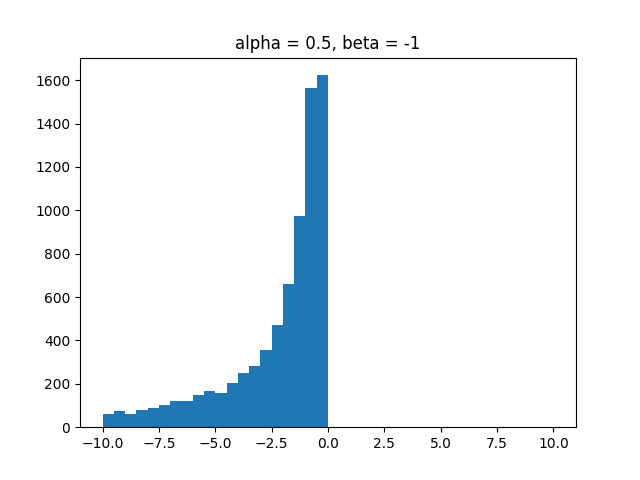
\includegraphics[width=0.3\textwidth]{q4_1_a0.5_bn1}
        \label{fig:q4_1_1}
    }
    \subfigure[$\alpha=0.5, \beta=-0.5$]{
        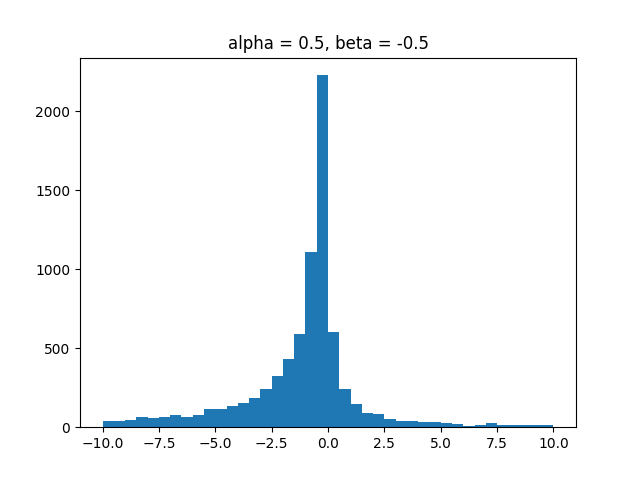
\includegraphics[width=0.3\textwidth]{q4_1_a0.5_bn0.5}
        \label{fig:q4_1_2}
    }
    \subfigure[$\alpha=0.5, \beta=0$]{
        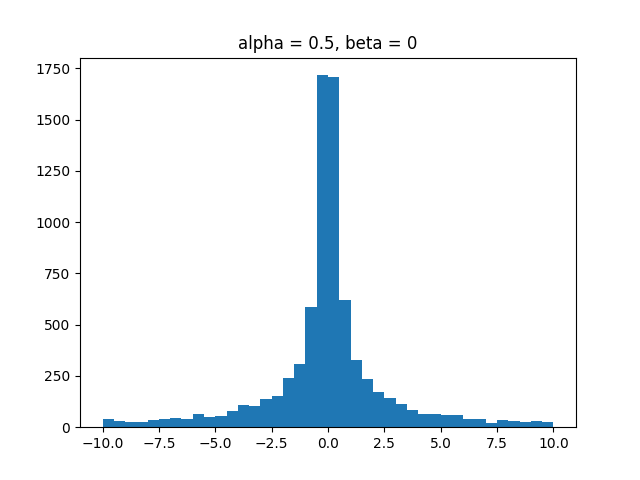
\includegraphics[width=0.3\textwidth]{q4_1_a0.5_b0}
        \label{fig:q4_1_3}
    }
    \subfigure[$\alpha=0.5, \beta=0.5$]{
        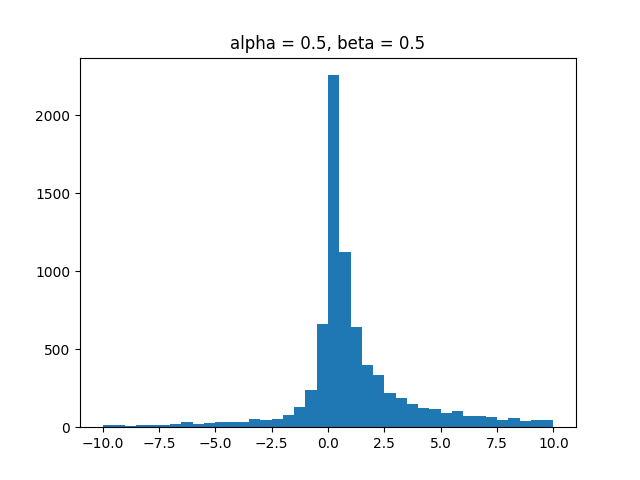
\includegraphics[width=0.3\textwidth]{q4_1_a0.5_b0.5}
        \label{fig:q4_1_4}
    }
    \subfigure[$\alpha=0.5, \beta=1$]{
        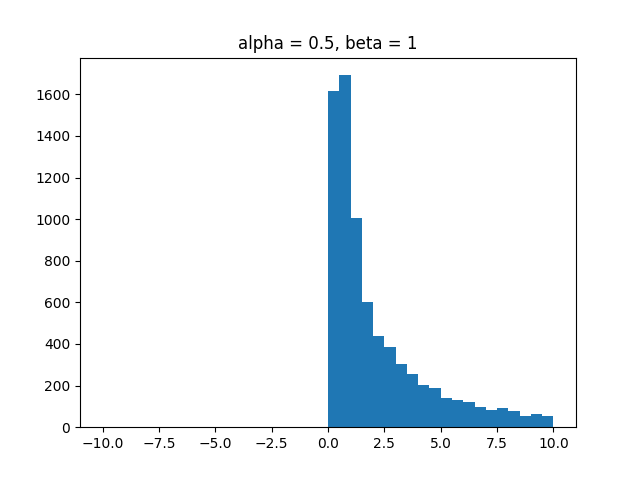
\includegraphics[width=0.3\textwidth]{q4_1_a0.5_b1}
        \label{fig:q4_1_5}
    }
    \caption{Histograms density estimates for $\alpha=0.5$ at $\beta \in \{-1, -0.5, 0, 0.5, 1\}$}
    \label{fig:q4_1_a0.5}
\end{figure}
\begin{figure}[htbp]
    \centering
    \subfigure[$\alpha=1.5, \beta=-1$]{
        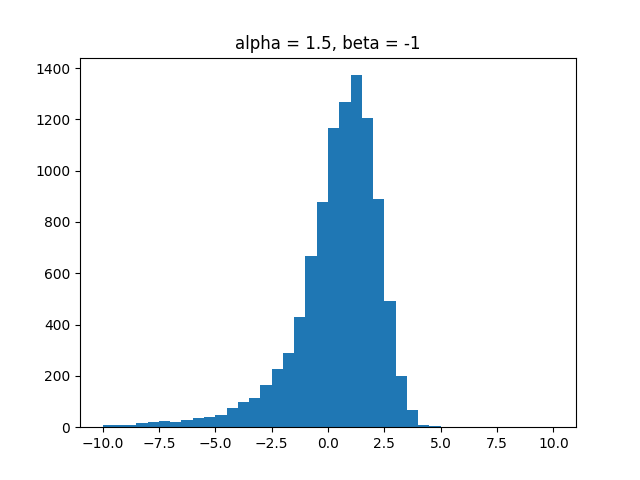
\includegraphics[width=0.3\textwidth]{q4_1_a1.5_bn1}
        \label{fig:q4_1_6}
    }
    \subfigure[$\alpha=1.5, \beta=-0.5$]{
        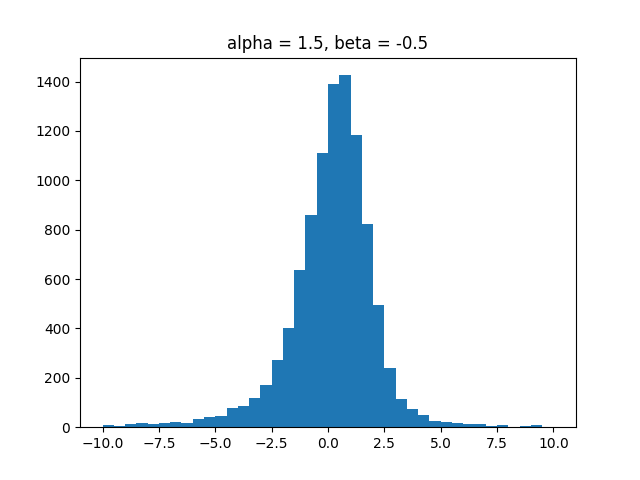
\includegraphics[width=0.3\textwidth]{q4_1_a1.5_bn0.5}
        \label{fig:q4_1_7}
    }
    \subfigure[$\alpha=1.5, \beta=0$]{
        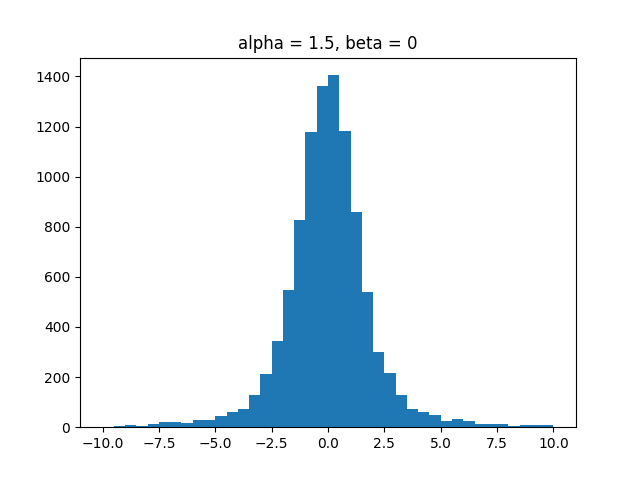
\includegraphics[width=0.3\textwidth]{q4_1_a1.5_b0}
        \label{fig:q4_1_8}
    }
    \subfigure[$\alpha=1.5, \beta=0.5$]{
        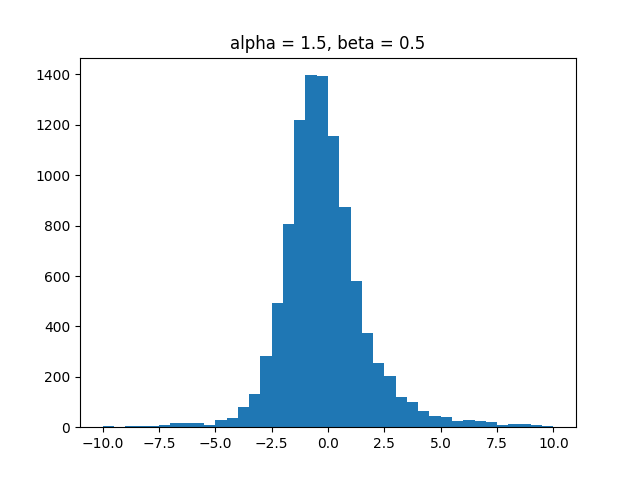
\includegraphics[width=0.3\textwidth]{q4_1_a1.5_b0.5}
        \label{fig:q4_1_9}
    }
    \subfigure[$\alpha=1.5, \beta=1$]{
        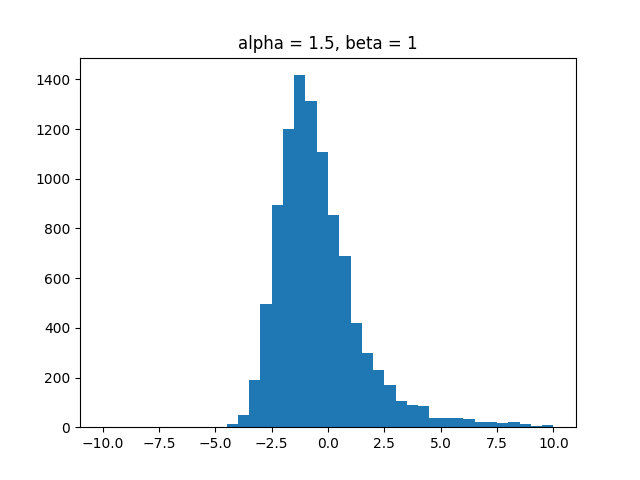
\includegraphics[width=0.3\textwidth]{q4_1_a1.5_b1}
        \label{fig:q4_1_10}
    }
    \caption{Histograms density estimates for $\alpha=1.5$ at $\beta \in \{-1, -0.5, 0, 0.5, 1\}$}
    \label{fig:q4_1_a1.5}
\end{figure}
\vspace{3in}

Hence comment on the interpretation of the parameters $\alpha$ and $\beta$.

\textcolor{darkblue}{
    Comparing the plots obtained for $\alpha=0.5$ and $\alpha=1.5$, it is observed that when $\alpha$ increase, the distribution becomes fuller and less steep, while a lower $\alpha$ value like 0.5 results in a sharp density peak centered around 0. Therefore $\alpha$ is likely to contribute to the \textbf{kurtosis} of the distribution, and a higher $\alpha$ value gives a lower kurtosis.\\
    \\
    Comparing the plots obtained for different values of $\beta$ that spread across the given permitted range of it, and as $\alpha$ is fixed, it is observed that $\beta$ controls the \textbf{skewness} of the sampled distribution. 
    A negative $\beta$ value results in a negatively-skewed distribution where the median is left of the mode(peak of histogram), and a positive $\beta$ value results in a positive skew where the median is on the right of the mode. At $\beta=0$, the sampled distribution of $x$ appears to be almost symmetrical around 0.0.
}

\end{enumerate}



\end{document}

